\chapter{Descripción de la solución propuesta}
Una vez que se sabe qué objetivos son los que se van a implementar en este TFG, lo primero que se debe realizar es un análisis exhaustivo de los mismos. Dicho análisis se va a hacer en base al estándar IEEE Std 830-1998 - IEEE Recommended Practice for Software Requirements Specifications \cite{IEE_830-1998}.
\\\\
Aunque el estándar anterior se remplazó por el estándar IEEE Std 830-1998 - IEEE Recommended Practice for Software Requirements Specifications \cite{IEE_29148-2011} enfocado a metodologías ágiles de creación de software, actualmente se sigue usando el antiguo estándar en multitud de proyectos empresariales y de la Administración Pública. Además, el antiguo es el que se explica en las asignaturas comunes del grado de informática \cite{guia-docente-fis} en esta escuela.
\\\\
A continuación se ha seguido parte del estándar IEEE Std 830-1998 \cite{IEE_830-1998} para analizar los objetivos específicos que se van a implementar en este TFG.
\section{Introducción}
Se va a proceder a la creación del núcleo principal de un sistema automático de gestión de aparcamientos para PMR (personas con movilidad reducida). Dicho sistema ayuda a la gestión de las plazas de aparcamiento, controla el estacionamiento en aquellas plazas que dispongan de sensores, alerta automáticamente cuando una plaza está siendo mal ocupada y guía al usuario a una plaza específica.
\section{Descripción del sistema actual}
Actualmente no existe un sistema automático para el control de plazas para PMR. El control se hace de forma manual y presencial en cada plaza.
\section{Objetivos}
En esta sección se exponen los objetivos del sistema que se quiere desarrollar. Dichos objetivos son:
\\\\
Para crear el sistema automático para el control de plazas para PMR, hay que crear la arquitectura del mismo. Esta arquitectura se ha detallado en el capítulo \ref{arquitectura} pero se detallará para esta solución posteriormente.
\begin{tabularx}{\textwidth}{|l|X|}
	\caption{Objetivo 1 del sistema}\label{OBJ-1}\\
	\hline
	OBJ-1        & Crear arquitectura del sistema \\ \hline
	Versión      & 1 (08/01/2018) \\ \hline
	Autores      & Carlos Cobos \\ \hline
	Descripción  & Se creará la estructura central para alojar al sistema. \\ \hline
	Subobjetivos & 	\begin{tabular}{@{}X@{}}
		OBJ-2 Crear aplicación de gestión (Tabla \ref{OBJ-2}). \\
		OBJ-6 Crear agente de captación de datos (Tabla \ref{OBJ-6}). \\
		OBJ-7 Crear aplicación móvil para el usuario final (Tabla \ref{OBJ-7}).
	\end{tabular} \\ \hline
	Comentarios  & \\ \hline
\end{tabularx}
Administrar el sistema dando de alta plazas de aparcamiento como acreditaciones de aparcamiento a la vez que, para poder recibir notificaciones de las plazas mal utilizadas, es necesario crear una aplicación que lo haga.
\begin{tabularx}{\textwidth}{|l|X|}
	\caption{Objetivo 2 del sistema}\label{OBJ-2}\\
	\hline
	OBJ-2        & Crear aplicación de gestión \\ \hline
	Versión      & 1 (08/01/2018) \\ \hline
	Autores      & Carlos Cobos \\ \hline
	Descripción  & El sistema deberá administrar y gestionar plazas de aparcamiento y acreditaciones. También deberá recibir notificaciones de ocupación de plazas. \\ \hline
	Subobjetivos & 	\begin{tabular}{@{}X@{}}
		OBJ-3 Recepcionar notificaciones (Tabla \ref{OBJ-3}). \\
		OBJ-4 Gestionar plazas de aparcamiento (Tabla \ref{OBJ-4}). \\ 
		OBJ-5 Gestionar acreditaciones de aparcamiento (Tabla \ref{OBJ-5}).
	\end{tabular} \\ \hline
	Comentarios  & \\ \hline
\end{tabularx}

\begin{tabularx}{\textwidth}{|l|X|}
	\caption{Objetivo 3 del sistema}\label{OBJ-3}\\
	\hline
	OBJ-3        & Recepcionar notificaciones \\ \hline
	Versión      & 1 (08/01/2018) \\ \hline
	Autores      & Carlos Cobos \\ \hline
	Descripción  & El sistema deberá notificar a los administradores cuando un vehículo sin autorización estacione en una plaza para PMR. \\ \hline
	Subobjetivos & 	\begin{tabular}{@{}X@{}}
		OBJ-6 Crear agente de captación de datos (Tabla \ref{OBJ-6}).
	\end{tabular} \\ \hline
	Comentarios  & \\ \hline
\end{tabularx}

\begin{tabularx}{\textwidth}{|l|X|}
	\caption{Objetivo 4 del sistema}\label{OBJ-4}\\
	\hline
	OBJ-4        & Gestionar plazas de aparcamiento \\ \hline
	Versión      & 1 (08/01/2018) \\ \hline
	Autores      & Carlos Cobos \\ \hline
	Descripción  & El sistema deberá guardar la información necesaria para la gestión de las distintas plazas de aparcamiento. Además, deberá permitir añadir nuevas plazas de aparcamiento, editar plazas y eliminar plazas existentes en el sistema. \\ \hline
	Subobjetivos & \\ \hline
	Comentarios  & \\ \hline
\end{tabularx}

\begin{tabularx}{\textwidth}{|l|X|}
	\caption{Objetivo 5 del sistema}\label{OBJ-5}\\
	\hline
	OBJ-5        & Gestionar acreditaciones de aparcamiento \\ \hline
	Versión      & 1 (08/01/2018) \\ \hline
	Autores      & Carlos Cobos \\ \hline
	Descripción  & El sistema deberá guardar la información necesaria para registrar los vehículos de aquellas personas que puedan aparcar en las plazas reservadas. Además, deberá permitir añadir nuevas acreditaciones de aparcamiento y eliminar existentes en el sistema. \\ \hline
	Subobjetivos & \\ \hline
	Comentarios  & \\ \hline
\end{tabularx}
Para mantener el sistema con los datos de aparcamiento actualizados es necesario un agente de captación de datos por cada plaza de aparcamiento que se encargue de monitorizar dicha plaza de aparcamiento asociada al agente y actualizar, cuando sea oportuno, los datos del sistema.
\newpage
\begin{tabularx}{\textwidth}{|l|X|}
	\caption{Objetivo 6 del sistema}\label{OBJ-6}\\
	\hline
	OBJ-6        & Crear agente de captación de datos \\ \hline
	Versión      & 1 (08/01/2018) \\ \hline
	Autores      & Carlos Cobos \\ \hline
	Descripción  & El sistema deberá alimentarse de información verídica y en tiempo real de las plazas de aparcamiento a través de agentes de captación de datos. Este va a ser un dispositivo hardware ubicado en las plazas de aparcamiento para PMR. \\ \hline
	Subobjetivos & \\ \hline
	Comentarios  & Éste agente de captación de datos se verá como un usuario que interactúa con el sistema. \\ \hline
\end{tabularx}
Por último, para que los usuarios de este tipo de plazas de aparcamiento se beneficien del sistema, se deberá crear una aplicación móvil para este tipo de usuarios donde poder ver y buscar una plaza de aparcamiento.
\begin{tabularx}{\textwidth}{|l|X|}
	\caption{Objetivo 7 del sistema}\label{OBJ-7}\\
	\hline
	OBJ-7        & Crear aplicación móvil para el usuario final \\ \hline
	Versión      & 1 (08/01/2018) \\ \hline
	Autores      & Carlos Cobos \\ \hline
	Descripción  & El sistema deberá servir información de plazas al usuario final. También deberá guiarle a plazas disponibles. \\ \hline
	Subobjetivos & 	\begin{tabular}{@{}X@{}}
		OBJ-8 Buscar plazas de aparcamiento (Tabla \ref{OBJ-8}).
	\end{tabular} \\ \hline
	Comentarios  & Este agente de captación de datos se verá como un usuario que interactúa con el sistema. \\ \hline
\end{tabularx}

\begin{tabularx}{\textwidth}{|l|X|}
	\caption{Objetivo 8 del sistema}\label{OBJ-8}\\
	\hline
	OBJ-8        & Buscar plazas de aparcamiento \\ \hline
	Versión      & 1 (08/01/2018) \\ \hline
	Autores      & Carlos Cobos \\ \hline
	Descripción  & El sistema deberá encontrar plazas de aparcamiento dado el destino del usuario final en base a la ocupación de las mismas. \\ \hline
	Subobjetivos & \\ \hline
	Comentarios  & \\ \hline
\end{tabularx}

\newpage
\section{Catálogo de requisitos del sistema}
Una vez que se han definido los objetivos globales del sistema, se va a proceder a definir qué información necesita guardar para funcionar correctamente, así como quién y cómo interactúa con el mismo.

\subsection{Requisitos de información}
Los requisitos de información describen qué tipo de información tiene que guardar el sistema para hacer frente a los objetivos marcados anteriormente. \\

\begin{tabularx}{\textwidth}{|l|X|}
	\caption{Requisito 1 de información del sistema}\label{IRQ-1}\\
	\hline
	IRQ-1                & Datos plaza de aparcamiento \\ \hline
	Versión              & 1 (09/01/2018) \\ \hline
	Autores              & Carlos Cobos \\ \hline
	Objetivos asociados  & 	{\begin{tabular}{@{}X@{}}
								OBJ-4 Gestionar plazas de aparcamiento (Tabla \ref{OBJ-4}).
							\end{tabular}} \\ \hline
	Requisitos asociados & IRQ-2 Datos ubicación de aparcamiento \\ \hline
	Descripción          & El sistema deberá almacenar la información correspondiente a las plazas de aparcamiento. En concreto: ubicación y estado actual. \\ \hline
	Datos específicos    & 	{\begin{tabular}{@{}X@{}}
								Puede haber más de una plaza con la misma ubicación. \\
								Ubicación: identificador de ubicación. \\
								Estado: número entero. -1 no definido, 0 disponible, 1 ocupada, 2 mal ocupada.
							\end{tabular}} \\ \hline
	Comentarios  & \\ \hline
\end{tabularx}

\begin{tabularx}{\textwidth}{|l|X|}
	\caption{Requisito 2 de información del sistema}\label{IRQ-2}\\
	\hline
	IRQ-2                & Datos ubicación de aparcamiento \\ \hline
	Versión              & 1 (09/01/2018) \\ \hline
	Autores              & Carlos Cobos \\ \hline
	Objetivos asociados  & 	\begin{tabular}{@{}X@{}}
		OBJ-4 Gestionar plazas de aparcamiento (Tabla \ref{OBJ-4}).
	\end{tabular} \\ \hline
	Requisitos asociados &  \\ \hline
	Descripción          & El sistema deberá almacenar la información correspondiente a las ubicaciones de las plazas de aparcamiento. En concreto: dirección, restricciones y plazas en dicha ubicación. \\ \hline
	Datos específicos    & 	{\begin{tabular}{@{}X@{}}
			Además de almacenar la calle y el número en la dirección, se debería almacenar su latitud y longitud (posición GPS) para geoposicionarla en un mapa. \\
			En algunas plazas hay restricciones horarias o posibilidad de que aparquen otros vehículos. \\
			Dirección: cadena de caracteres. Calle y número. \\
			Latitud: número decimal. \\
			Longitud: numero decimal. \\
			Restricciones: cadena compleja. \\
			Número de plazas totales: número entero.
	\end{tabular}} \\ \hline
	Comentarios  & \\ \hline
\end{tabularx}

\begin{tabularx}{\textwidth}{|l|X|}
	\caption{Requisito 3 de información del sistema}\label{IRQ-3}\\
	\hline
	IRQ-3                & Datos acreditación de aparcamiento \\ \hline
	Versión              & 1 (09/01/2018) \\ \hline
	Autores              & Carlos Cobos \\ \hline
	Objetivos asociados  & 	\begin{tabular}{@{}X@{}}
		OBJ-5 Gestionar acreditaciones de aparcamiento (Tabla \ref{OBJ-5}).
	\end{tabular} \\ \hline
	Requisitos asociados &  \\ \hline
	Descripción          & El sistema deberá almacenar la información correspondiente a las acreditaciones de aparcamiento. En concreto: identificador de acreditación. \\ \hline
	Datos específicos    & 	{\begin{tabular}{@{}X@{}}
			Cada acreditación pertenece a una persona registrada en un sistema externo. \\
			Una persona física solamente puede poseer una acreditación activa.\\
			Identificador acreditación: número entero. Normalmente almacenado en hexadecimal.
	\end{tabular}} \\ \hline
	Comentarios  & \\ \hline
\end{tabularx}

\newpage
\begin{tabularx}{\textwidth}{|l|X|}
	\caption{Requisito 4 de información del sistema}\label{IRQ-4}\\
	\hline
	IRQ-4                & Registro de utilización de plazas \\ \hline
	Versión              & 1 (09/01/2018) \\ \hline
	Autores              & Carlos Cobos \\ \hline
	Objetivos asociados  & 	{\begin{tabular}{@{}X@{}}
		OBJ-4 Gestionar plazas de aparcamiento (Tabla \ref{OBJ-4}). \\
		OBJ-6 Crear agente de captación de datos (Tabla \ref{OBJ-6}). \\
		OBJ-8 Buscar mejores plazas de aparcamiento (Tabla \ref{OBJ-8}). \\
		OBJ-FUTURO Preparación de datos para estadísticas de plazas.
	\end{tabular}} \\ \hline
	Requisitos asociados &  \\ \hline
	Descripción          & El sistema deberá almacenar la información correspondiente al estado de las plazas en el transcurso del tiempo. \\ \hline
	Datos específicos    & 	{\begin{tabular}{@{}X@{}}
			Se almacenará el identificador de la plaza junto al nuevo estado que haya tomado y la fecha y hora cuando una plaza cambie de estado. \\
			El agente de captación de datos notificará al sistema cuando ocurra un cambio de estado en su plaza. \\
			Identificador de plaza: número entero. \\
			Estado: número entero. -1 no definido, 0 disponible, 1 ocupada, 2 mal ocupada. \\
			Tiempo: marca de tiempo (fecha y hora).
	\end{tabular}} \\ \hline
	Comentarios  & \\ \hline
\end{tabularx}

\begin{tabularx}{\textwidth}{|l|X|}
	\caption{Requisito 5 de información del sistema}\label{IRQ-5}\\
	\hline
	IRQ-5                & Registro de destino de usuarios \\ \hline
	Versión              & 1 (09/01/2018) \\ \hline
	Autores              & Carlos Cobos \\ \hline
	Objetivos asociados  & 	{\begin{tabular}{@{}X@{}}
			OBJ-8 Buscar mejores plazas de aparcamiento (Tabla \ref{OBJ-8}). \\
			OBJ-FUTURO Preparación de datos para estadísticas de plazas. \\
			OBJ-FUTURO Preparación de datos para estadísticas de destino.
	\end{tabular}} \\ \hline
	Requisitos asociados &  \\ \hline
	Descripción          & El sistema deberá almacenar la información correspondiente al destino de los usuarios. \\ \hline
	Datos específicos    & 	{\begin{tabular}{@{}X@{}}
			Se almacenará el destino que busca un usuario junto a la marca de tiempo en el que se ha producido la búsqueda. \\
			Latitud: número decimal. Latitud del destino final del usuario. \\
			Longitud: numero decimal. Longitud del destino final del usuario. \\
			Tiempo: marca de tiempo (fecha y hora). 
	\end{tabular}} \\ \hline
	Comentarios  & Por ahora y debido a que una acreditación representa únicamente a un usuario, se tomará el identificador de la acreditación como el del usuario. \\ \hline
\end{tabularx}

\begin{tabularx}{\textwidth}{|l|X|}
	\caption{Requisito 6 de información del sistema}\label{IRQ-6}\\
	\hline
	IRQ-6                & Destino activo \\ \hline
	Versión              & 1 (09/01/2018) \\ \hline
	Autores              & Carlos Cobos \\ \hline
	Objetivos asociados  & 	{\begin{tabular}{@{}X@{}}
			OBJ-7 Crear aplicación móvil para el usuario final (Tabla \ref{OBJ-7}). \\
			OBJ-8 Buscar mejores plazas de aparcamiento (Tabla \ref{OBJ-8}). \\
	\end{tabular}} \\ \hline
	Requisitos asociados &  \\ \hline
	Descripción          & Para que el sistema sepa a quién notificar al ocuparse una plaza de aparcamiento, deberá almacenar la información correspondiente a la ubicación de destino de los usuarios de la aplicación móvil desde el momento que inicia la navegación a dicha ubicación hasta que llega al destino o interrumpe la navegación. \\ \hline
	Datos específicos    & 	{\begin{tabular}{@{}X@{}}
			Identificador de la aplicación móvil del usuario: número entero. \\
			Identificador de la ubicación de destino: número entero. \\
	\end{tabular}} \\ \hline
	Comentarios  & Dicha información sirve para avisar al posible usuario, que está navegando a una ubicación determinada, si la última plaza libre de ésta se ha ocupado. \\ \hline
\end{tabularx}

\newpage
\subsubsection{Requisitos funcionales}
Los requisitos funcionales describen las acciones del sistema. Para que pueda realizar algunas de las mismas, se tiene que definir a los usuarios que interactúan con éste. Estos usuarios, en adelante actores, ordenan lo que el sistema tiene que hacer pidiendo datos que el actor tiene que introducir. A esta interacción se le llama \textit{caso de uso}.
\begin{tabularx}{\textwidth}{|l|X|}
	\caption{Requisito funcional 1 del sistema}\label{FR-1}\\
	\hline
	FR-1        & Administrar ubicaciones de aparcamiento \\ \hline
	Versión     & 1 (10/01/2018) \\ \hline
	Autores     & Carlos Cobos \\ \hline
	Descripción & Los administradores deberán dar de alta, modificar o eliminar ubicaciones del sistema. \\ \hline
	Comentarios &  \\ \hline
\end{tabularx}

\begin{tabularx}{\textwidth}{|l|X|}
	\caption{Requisito funcional 2 del sistema}\label{FR-2}\\
	\hline
	FR-2        & Administrar plazas de aparcamiento \\ \hline
	Versión     & 1 (10/01/2018) \\ \hline
	Autores     & Carlos Cobos \\ \hline
	Descripción & Los administradores deberán dar de alta o de baja plazas de las ubicaciones del sistema. \\ \hline
	Comentarios &  \\ \hline
\end{tabularx}

\begin{tabularx}{\textwidth}{|l|X|}
	\caption{Requisito funcional 3 del sistema}\label{FR-3}\\
	\hline
	FR-3        & Administrar acreditaciones de aparcamiento \\ \hline
	Versión     & 1 (10/01/2018) \\ \hline
	Autores     & Carlos Cobos \\ \hline
	Descripción & Los administradores deberán dar de alta o de baja acreditaciones de aparcamiento del sistema. \\ \hline
	Comentarios &  \\ \hline
\end{tabularx}

\begin{tabularx}{\textwidth}{|l|X|}
	\caption{Requisito funcional 4 del sistema}\label{FR-4}\\
	\hline
	FR-4        & Actualizar estado de las plazas \\ \hline
	Versión     & 1 (10/01/2018) \\ \hline
	Autores     & Carlos Cobos \\ \hline
	Descripción & Los agentes de captación deberán actualizar la plaza asociada en el sistema. \\ \hline
	Comentarios &  \\ \hline
\end{tabularx}

\newpage
\begin{tabularx}{\textwidth}{|l|X|}
	\caption{Requisito funcional 5 del sistema}\label{FR-5}\\
	\hline
	FR-5        & Gestionar notificaciones \\ \hline
	Versión     & 1 (10/01/2018) \\ \hline
	Autores     & Carlos Cobos \\ \hline
	Descripción & Los administradores deberán recibir un aviso cuando una plaza sea mal usada. Por su parte, el usuario deberá recibir un aviso cuando se ocupen todas las plazas de la ubicación a la que se dirige. \\ \hline
	Comentarios &  \\ \hline
\end{tabularx}

\begin{tabularx}{\textwidth}{|l|X|}
	\caption{Requisito funcional 6 del sistema}\label{FR-6}\\
	\hline
	FR-6        & Buscar plazas \\ \hline
	Versión     & 1 (10/01/2018) \\ \hline
	Autores     & Carlos Cobos \\ \hline
	Descripción & El sistema deberá mostrar una lista de ubicaciones donde se pueda aparcar dada una posición. \\ \hline
	Comentarios &  \\ \hline
\end{tabularx}

\begin{tabularx}{\textwidth}{|l|X|}
	\caption{Requisito funcional 7 del sistema}\label{FR-7}\\
	\hline
	FR-7        & Navegar a plazas de aparcamiento \\ \hline
	Versión     & 1 (10/01/2018) \\ \hline
	Autores     & Carlos Cobos \\ \hline
	Descripción & El sistema deberá guiar al usuario a una ubicación de aparcamiento. \\ \hline
	Comentarios &  \\ \hline
\end{tabularx}

\newpage
\subsubsection{Definición de los actores}
\begin{tabularx}{\textwidth}{|l|X|}
	\caption{Actor 1 del sistema}\label{ACT-1}\\
	\hline
	ACT-1       & Usuario final \\ \hline
	Versión     & 1 (10/01/2018) \\ \hline
	Autores     & Carlos Cobos \\ \hline
	Descripción & Este actor representa al usuario final del sistema que desea hacer uso de las plazas monitorizadas. \\ \hline
	Comentarios & Este actor hará uso del sistema a través de una aplicación móvil cuando se encuentre en el vehículo. \\ \hline
\end{tabularx}

\begin{tabularx}{\textwidth}{|l|X|}
	\caption{Actor 2 del sistema}\label{ACT-2}\\
	\hline
	ACT-2       & Administrador \footnotemark \\ \hline
	Versión     & 1 (10/01/2018) \\ \hline
	Autores     & Carlos Cobos \\ \hline
	Descripción & Este actor representa a varios de los posibles administradores en un futuro. Este actor podrá gestionar todo el sistema. \\ \hline
	Comentarios & Este actor hará uso del sistema a través de una aplicación de escritorio. \\ \hline
\end{tabularx}

\footnotetext{En un futuro, este actor de dividirá en tres: agentes de administración local, agentes de la autoridad local y agentes de la administración regional.}
\begin{tabularx}{\textwidth}{|l|X|}
	\caption{Actor 3 del sistema}\label{ACT-3}\\
	\hline
	ACT-3       & Agente de captación de datos \\ \hline
	Versión     & 1 (10/01/2018) \\ \hline
	Autores     & Carlos Cobos \\ \hline
	Descripción & Este actor representa a los dispositivos que se colocarán en las plazas de aparcamiento para proveer al sistema de datos. \\ \hline
	Comentarios & Este actor será un dispositivo electrónico. \\ \hline
\end{tabularx}

\newpage
\subsubsection{Casos de uso}
%\begin{figure}[H]
%	\centering
%	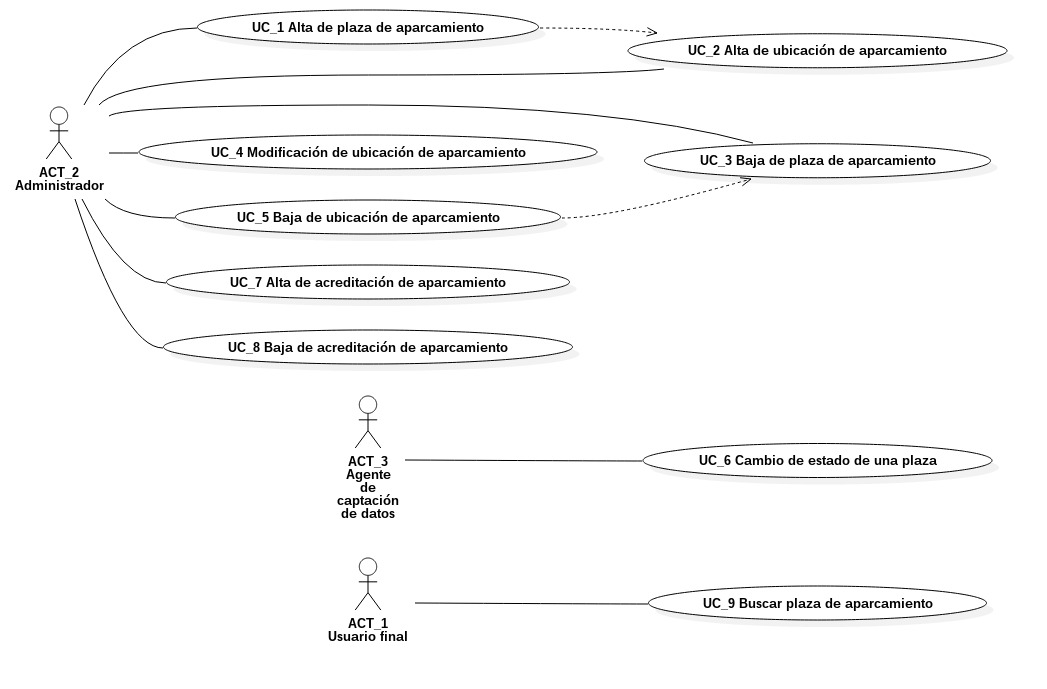
\includegraphics[width=\textwidth]{imagenes/casos_de_uso.jpg}
%	\caption{Esquema casos de uso}
%	\label{esquema_UC}
%\end{figure}

\begin{sidewaysfigure}[H]
	\centering
	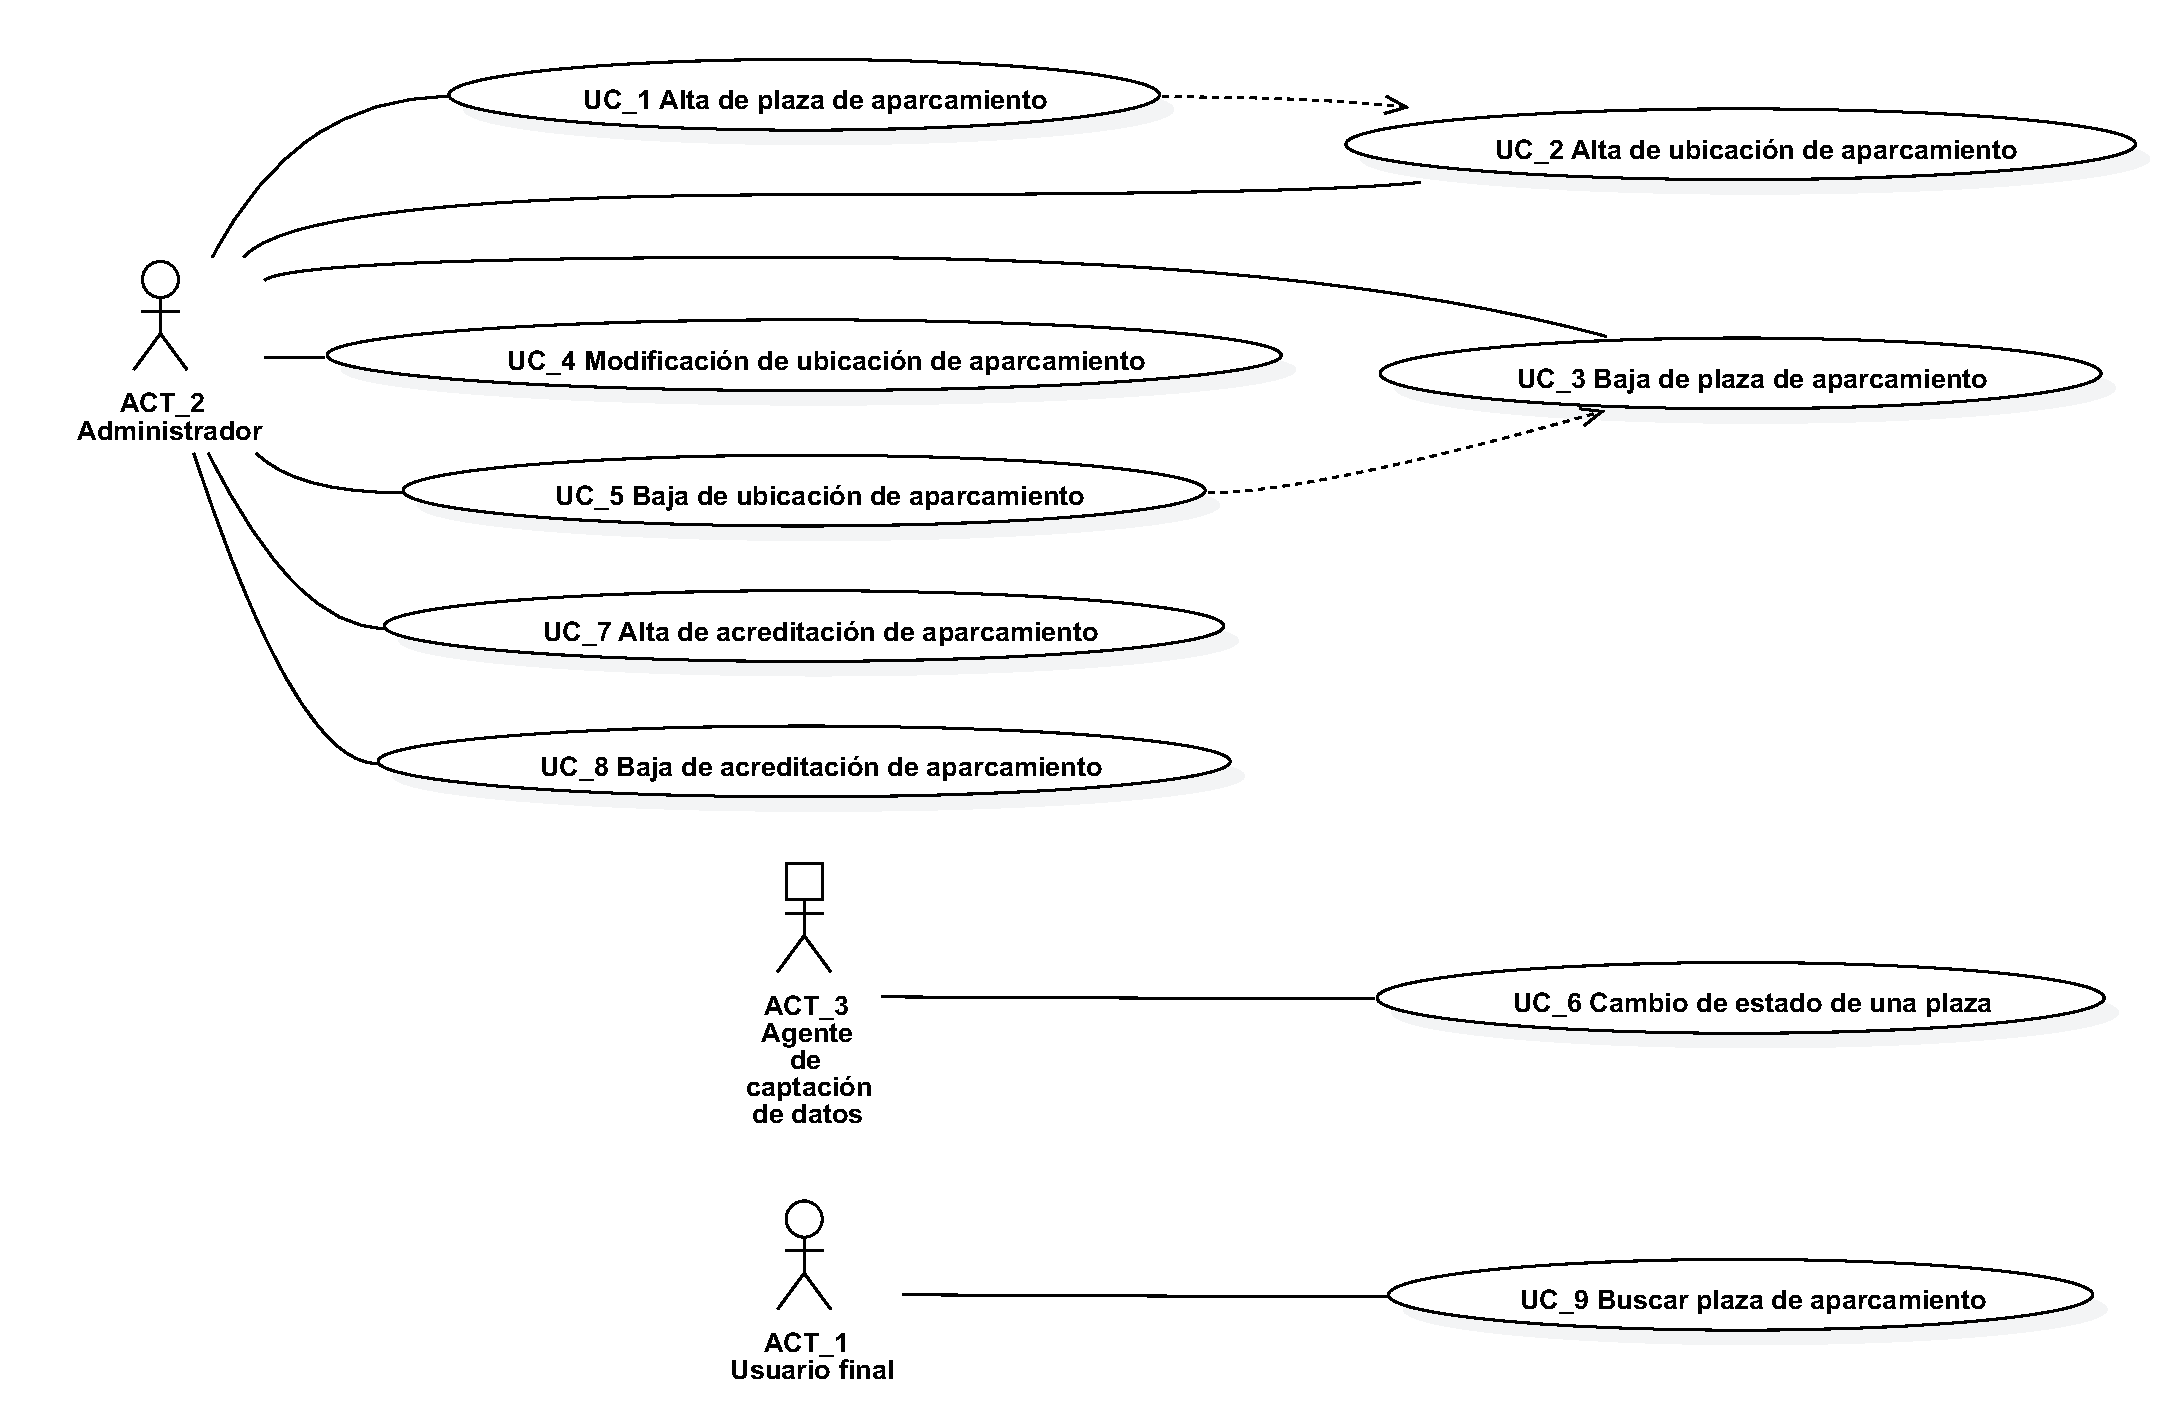
\includegraphics[width=\textwidth]{imagenes/casos_de_uso.eps}
	\caption{Esquema casos de uso}
	\label{esquema_UC}
\end{sidewaysfigure}

\begin{tabularx}{\textwidth}{|l|X|}
	\caption{Caso de uso 1 del sistema}\label{UC-1}\\
	\hline
	UC-1                 & Alta de plaza de aparcamiento \\ \hline
	Versión              & 1 (10/01/2018) \\ \hline
	Autores              & Carlos Cobos \\ \hline
	Objetivos asociados  & OBJ-4 Gestionar plazas de aparcamiento (Tabla \ref{OBJ-4} \\ \hline
	Requisitos asociados &  {\begin{tabular}{@{}X@{}}
									IRQ-1 Datos plaza de aparcamiento (Tabla \ref{IRQ-1}) \\
									IRQ-2 Datos ubicación de aparcamiento (Tabla \ref{IRQ-2}) \\
									FR-2 Administrar plazas de aparcamiento (Tabla \ref{FR-2}) \\
							\end{tabular}} \\ \hline
	Descripción          & El sistema deberá pedir los datos necesarios al administrador para añadir una nueva plaza de aparcamiento en el sistema. \\ \hline
	Precondición         &  \\ \hline
	Secuencia normal     & 	{\begin{tabular}{@{}l|p{\anchoColumna{}}@{}}
								Paso & Acción \\ \hline
								1 & El actor administrador inserta un identificador de una ubicación. \\ \hline
								2 & El sistema añade una plaza a la ubicación dada. \\ \hline
								3 & El sistema actualiza el número de plazas de la ubicación dada. \\
							\end{tabular}} \\ \hline
	Postcondición        &  \\ \hline
	Excepciones          & 	{\begin{tabular}{@{}l|p{\anchoColumna{}}@{}}
								Paso & Acción \\ \hline
								1 & Si la ubicación de la nueva plaza no existe, se realizará el caso de uso UC-2 (Tabla \ref{UC-2}). \\
							\end{tabular}} \\ \hline
\end{tabularx}

\begin{tabularx}{\textwidth}{|l|X|}
	\caption{Caso de uso 2 del sistema}\label{UC-2}\\
	\hline
	UC-2                 & Alta de ubicación de aparcamiento \\ \hline
	Versión              & 1 (10/01/2018) \\ \hline
	Autores              & Carlos Cobos \\ \hline
	Objetivos asociados  & 	{\begin{tabular}{@{}X@{}}
			OBJ-4 Gestionar plazas de aparcamiento (Tabla \ref{OBJ-4}) \\
	\end{tabular}} \\ \hline
	Requisitos asociados &  {\begin{tabular}{@{}X@{}}
			IRQ-2 Datos ubicación de aparcamiento (Tabla \ref{IRQ-2}) \\
			FR-2 Administrar plazas de aparcamiento (Tabla \ref{FR-2}) \\
	\end{tabular}} \\ \hline
	Descripción          & El sistema deberá pedir los datos necesarios al administrador para añadir una nueva ubicación de aparcamiento en el sistema. \\ \hline
	Precondición         &  \\ \hline
	Secuencia normal     & 	{\begin{tabular}{@{}l|p{\anchoColumna{}}@{}}
			Paso & Acción \\ \hline
			1 & El actor administrador introduce una dirección, una posición GPS (latitud y longitud) y unas restricciones a la ubicación si precede. \\ \hline
			2 & El sistema añade la nueva ubicación con número de plazas a 0. \\
	\end{tabular}} \\ \hline
	Postcondición        &  \\ \hline
	Excepciones          & 	{\begin{tabular}{@{}l|p{\anchoColumna{}}@{}}
			Paso & Acción \\ \hline
			1 & Si la posición GPS de la plaza es igual que la de una plaza existente en el sistema, no se procederá.
	\end{tabular}} \\ \hline
\end{tabularx}

\begin{tabularx}{\textwidth}{|l|X|}
	\caption{Caso de uso 3 del sistema}\label{UC-3}\\
	\hline
	UC-3                 & Baja de plaza de aparcamiento \\ \hline
	Versión              & 1 (10/01/2018) \\ \hline
	Autores              & Carlos Cobos \\ \hline
	Objetivos asociados  & 	{\begin{tabular}{@{}X@{}}
			OBJ-4 Gestionar plazas de aparcamiento (Tabla \ref{OBJ-4}) \\
	\end{tabular}} \\ \hline
	Requisitos asociados &  {\begin{tabular}{@{}X@{}}
			IRQ-1 Datos plaza de aparcamiento (Tabla \ref{IRQ-1}) \\
			IRQ-2 Datos ubicación de aparcamiento (Tabla \ref{IRQ-2}) \\
			FR-2 Administrar plazas de aparcamiento (Tabla \ref{FR-2}) \\
	\end{tabular}} \\ \hline
	Descripción          & El sistema deberá pedir los datos necesarios al administrador para eliminar una plaza de aparcamiento en el sistema. \\ \hline
	Precondición         &  \\ \hline
	Secuencia normal     & 	{\begin{tabular}{@{}l|p{\anchoColumna{}}@{}}
			Paso & Acción \\ \hline
			1 & El actor administrador inserta un identificador de una plaza. \\ \hline
			2 & El sistema elimina la plaza seleccionada. \\ \hline
			3 & El sistema actualiza el número de plazas de la ubicación asociada. \\
	\end{tabular}} \\ \hline
	Postcondición        &  \\ \hline
	Excepciones          & 	{\begin{tabular}{@{}l|p{\anchoColumna{}}@{}}
			Paso & Acción \\ \hline
			1 & Si el identificador de la plaza no existe, no se procederá. \\ 
	\end{tabular}} \\ \hline
\end{tabularx}

\newpage
\begin{tabularx}{\textwidth}{|l|X|}
	\caption{Caso de uso 4 del sistema}\label{UC-4}\\
	\hline
	UC-4                 & Modificación de ubicación de aparcamiento \\ \hline
	Versión              & 1 (10/01/2018) \\ \hline
	Autores              & Carlos Cobos \\ \hline
	Objetivos asociados  & 	{\begin{tabular}{@{}X@{}}
			OBJ-4 Gestionar plazas de aparcamiento (Tabla \ref{OBJ-4}) \\
	\end{tabular}} \\ \hline
	Requisitos asociados &  {\begin{tabular}{@{}X@{}}
			IRQ-2 Datos ubicación de aparcamiento (Tabla \ref{IRQ-2}) \\
			FR-1 Administrar ubicaciones de aparcamiento (Tabla \ref{FR-1}) \\
	\end{tabular}} \\ \hline
	Descripción          & El sistema deberá permitir modificar algunos campos de la ubicación de plazas. \\ \hline
	Precondición         &  \\ \hline
	Secuencia normal     & 	{\begin{tabular}{@{}l|p{\anchoColumna{}}@{}}
			Paso & Acción \\ \hline
			1 & El actor administrador inserta un identificador de una ubicación. \\ \hline
			2 & El sistema muestra la información asociada a dicha ubicación. \\ \hline
			3 & El actor administrador podrá modificar la dirección y las restricciones de la ubicación. \\ \hline
			4 & El sistema almacenará la nueva información. \\
	\end{tabular}} \\ \hline
	Postcondición        &  \\ \hline
	Excepciones          & 	{\begin{tabular}{@{}l|p{\anchoColumna{}}@{}}
			Paso & Acción \\ \hline
			1 & Si el identificador de la ubicación no existe, no se procederá. \\ 
	\end{tabular}} \\ \hline
\end{tabularx}

\begin{tabularx}{\textwidth}{|l|X|}
	\caption{Caso de uso 5 del sistema}\label{UC-5}\\
	\hline
	UC-5                 & Baja de ubicación de aparcamiento \\ \hline
	Versión              & 1 (10/01/2018) \\ \hline
	Autores              & Carlos Cobos \\ \hline
	Objetivos asociados  & 	{\begin{tabular}{@{}X@{}}
			OBJ-4 Gestionar plazas de aparcamiento (Tabla \ref{OBJ-4}) \\
	\end{tabular}} \\ \hline
	Requisitos asociados &  {\begin{tabular}{@{}X@{}}
			IRQ-2 Datos ubicación de aparcamiento (Tabla \ref{IRQ-2}) \\
			FR-1 Administrar ubicaciones de aparcamiento (Tabla \ref{FR-1}) \\
	\end{tabular}} \\ \hline
	Descripción          & El sistema deberá permitir eliminar una ubicación de plazas. \\ \hline
	Precondición         &  \\ \hline
	Secuencia normal     & 	{\begin{tabular}{@{}l|p{\anchoColumna{}}@{}}
			Paso & Acción \\ \hline
			1 & El actor administrador inserta un identificador de una ubicación. \\ \hline
			2 & El sistema muestra la información asociada a dicha ubicación. \\ \hline
			3 & El actor administrador confirmará la ubicación. \\ \hline
			4 & El sistema eliminará la ubicación. \\ 
	\end{tabular}} \\ \hline
	Postcondición        &  \\ \hline
	Excepciones          & 	{\begin{tabular}{@{}l|p{\anchoColumna{}}@{}}
			Paso & Acción \\ \hline
			1 & Si el identificador de la ubicación no existe, no se procederá. \\ \hline
			3 & Si el número de plazas totales de la ubicación es mayor de 0, no se procederá. \\
	\end{tabular}} \\ \hline
\end{tabularx}

\begin{tabularx}{\textwidth}{|l|X|}
	\caption{Caso de uso 6 del sistema}\label{UC-6}\\
	\hline
	UC-6                 & Cambio de estado de una plaza \\ \hline
	Versión              & 1 (10/01/2018) \\ \hline
	Autores              & Carlos Cobos \\ \hline
	Objetivos asociados  & 	{\begin{tabular}{@{}X@{}}
			OBJ-3 Recepcionar notificaciones (Tabla \ref{OBJ-3}) \\
			OBJ-4 Gestionar plazas de aparcamiento (Tabla \ref{OBJ-4}) \\
			OBJ-6 Crear agente de captación de datos (Tabla \ref{OBJ-6})
	\end{tabular}} \\ \hline
	Requisitos asociados &  {\begin{tabular}{@{}X@{}}
			IRQ-1 Datos plaza de aparcamiento (Tabla \ref{IRQ-1}) \\
			IRQ-2 Datos ubicación de aparcamiento (Tabla \ref{IRQ-2}) \\
			IRQ-3 Datos acreditación de aparcamiento (Tabla \ref{IRQ-3}) \\
			IRQ-4 Registro de utilización de plazas (Tabla \ref{IRQ-4}) \\
			IRQ-6 Destino activo (Tabla \ref{IRQ-3}) \\
			FR-4 Actualizar estado de las plazas (Tabla \ref{FR-4}) \\
			FR-5 Gestionar notificaciones (Tabla \ref{FR-5}) \\
	\end{tabular}} \\ \hline
	Descripción          & Cuando el agente de captación de datos detecte un cambio de estado en su plaza, el sistema deberá almacenar dicho estado y actuar en consecuencia. \\ \hline
	Precondición         &  \\ \hline
	Secuencia normal     & 	{\begin{tabular}{@{}l|p{\anchoColumna{}}@{}}
			Paso & Acción \\ \hline
			1 & El agente de captación de datos detecta un cambio de estado en su plaza. \\ \hline
			2 & {\begin{tabular}{@{}l|p{\anchoColumnaInterior{}}@{}}
					& Si la plaza se ha quedado libre. \\ \hline
					2.1 & El sistema actualiza los datos de la plaza de aparcamiento. \\ \hline
					2.2 & El sistema actualiza los datos del registro de utilización de la plaza de aparcamiento. \\
				\end{tabular}} \\ \hline
			3 & {\begin{tabular}{@{}l|p{\anchoColumnaInterior{}}@{}}
					& Si la plaza se ha quedado ocupada. \\ \hline
					3.1 & El sistema lee la acreditación del vehículo. \\ \hline
					3.2 & {\begin{tabular}{@{}l|p{\anchoColumnaMasInterior{}}@{}}
							& El sistema comprueba que la plaza no esté en el registro de destino activo. \\ \hline
							3.2.1 & Si está, se notifica a la aplicación móvil asociada. \\
						\end{tabular}} \\ 
					3.3 & El sistema comprueba que la acreditación leída existe. \\ \hline
					3.4 & El sistema actualiza los datos de la plaza de aparcamiento. \\ \hline
					3.5 & El sistema actualiza los datos del registro de utilización de la plaza de aparcamiento. \\
				\end{tabular}} \\ 
	\end{tabular}} \\ \hline
	Postcondición        &  \\ \hline
	Excepciones          & 	{\begin{tabular}{@{}l|p{\anchoColumna{}}@{}}
			Paso & Acción \\ \hline
			3.1 & {\begin{tabular}{@{}l|p{\anchoColumnaInterior{}}@{}}
					& No se detecta acreditación del vehículo. \\ \hline
					1 & Se notifica a la aplicación de administración sobre la incidencia. \\ \hline
					2 & El sistema actualiza los datos de la plaza de aparcamiento con estado mal ocupado. \\ \hline
					3 & El sistema actualiza los datos del registro de utilización de la plaza de aparcamiento. \\
				\end{tabular}} \\ \hline
			3.3 & {\begin{tabular}{@{}l|p{\anchoColumnaInterior{}}@{}}
					& La acreditación leída no existe en el sistema. \\ \hline
					1 & Se notifica a la aplicación de administración sobre la incidencia. \\ \hline
					2 & El sistema actualiza los datos de la plaza de aparcamiento con estado mal ocupado. \\ \hline
					3 & El sistema actualiza los datos del registro de utilización de la plaza de aparcamiento. \\
			\end{tabular}}
	\end{tabular}} \\ \hline
\end{tabularx}

\begin{tabularx}{\textwidth}{|l|X|}
	\caption{Caso de uso 7 del sistema}\label{UC-7}\\
	\hline
	UC-7                 & Alta de acreditación de aparcamiento \\ \hline
	Versión              & 1 (10/01/2018) \\ \hline
	Autores              & Carlos Cobos \\ \hline
	Objetivos asociados  & 	{\begin{tabular}{@{}X@{}}
			OBJ-5 Gestionar acreditaciones de aparcamiento (Tabla \ref{OBJ-5}) \\
	\end{tabular}} \\ \hline
	Requisitos asociados &  {\begin{tabular}{@{}X@{}}
			IRQ-3 Datos acreditación de aparcamiento (Tabla \ref{IRQ-3}) \\
			FR-3 Administrar acreditaciones de aparcamiento (Tabla \ref{FR-3}) \\
	\end{tabular}} \\ \hline
	Descripción          & El sistema deberá pedir los datos necesarios al administrador para añadir una nueva acreditación de aparcamiento en el sistema. \\ \hline
	Precondición         & Identificador de la nueva acreditación no existe en el sistema. \\ \hline
	Secuencia normal     & 	{\begin{tabular}{@{}l|p{\anchoColumna{}}@{}}
			Paso & Acción \\ \hline
			1 & El actor administrador introduce un nuevo identificador único de acreditación. \\ \hline
			2 & El sistema añade la nueva acreditación. \\
	\end{tabular}} \\ \hline
	Postcondición        &  \\ \hline
	Excepciones          & 	{\begin{tabular}{@{}l|p{\anchoColumna{}}@{}}
			Paso & Acción \\ \hline
			1 & Si la posición GPS de la plaza es igual que la de una plaza existente en el sistema, no se procederá.
	\end{tabular}} \\ \hline
\end{tabularx}

\begin{tabularx}{\textwidth}{|l|X|}
	\caption{Caso de uso 8 del sistema}\label{UC-8}\\
	\hline
	UC-8                 & Baja de acreditación de aparcamiento \\ \hline
	Versión              & 1 (10/01/2018) \\ \hline
	Autores              & Carlos Cobos \\ \hline
	Objetivos asociados  & 	{\begin{tabular}{@{}X@{}}
			OBJ-5 Gestionar acreditaciones de aparcamiento (Tabla \ref{OBJ-5}) \\
	\end{tabular}} \\ \hline
	Requisitos asociados &  {\begin{tabular}{@{}X@{}}
			IRQ-3 Datos acreditación de aparcamiento (Tabla \ref{IRQ-3}) \\
			FR-3 Administrar acreditaciones de aparcamiento (Tabla \ref{FR-3}) \\
	\end{tabular}} \\ \hline
	Descripción          & El sistema deberá pedir los datos necesarios al administrador para eliminar una acreditación de aparcamiento del sistema. \\ \hline
	Precondición         & Identificador de la acreditación existe en el sistema. \\ \hline
	Secuencia normal     & 	{\begin{tabular}{@{}l|p{\anchoColumna{}}@{}}
			Paso & Acción \\ \hline
			1 & El actor administrador introduce un identificador único de acreditación. \\ \hline
			2 & El actor administrador confirma el identificador. \\ \hline
			3 & El sistema borra la acreditación. \\
	\end{tabular}} \\ \hline
	Postcondición        &  \\ \hline
	Excepciones          & 	{\begin{tabular}{@{}l|p{\anchoColumna{}}@{}}
			Paso & Acción \\ \hline
			1 & Si la posición GPS de la plaza es igual que la de una plaza existente en el sistema, no se procederá.
	\end{tabular}} \\ \hline
\end{tabularx}

\begin{tabularx}{\textwidth}{|l|X|}
	\caption{Caso de uso 9 del sistema}\label{UC-9}\\
	\hline
	UC-9                 & Buscar plaza de aparcamiento \\ \hline
	Versión              & 1 (10/01/2018) \\ \hline
	Autores              & Carlos Cobos \\ \hline
	Objetivos asociados  & 	{\begin{tabular}{@{}X@{}}
			OBJ-8 Buscar plazas de aparcamiento (Tabla \ref{OBJ-8}) \\
	\end{tabular}} \\ \hline
	Requisitos asociados &  {\begin{tabular}{@{}X@{}}
			IRQ-1 Datos plaza de aparcamiento (Tabla \ref{IRQ-3}) \\
			IRQ-4 Registro de utilización de plazas (Tabla \ref{IRQ-4}) \\
			IRQ-5 Registro de destino de usuarios (Tabla \ref{IRQ-5}) \\
			FR-6 Buscar plazas (Tabla \ref{FR-6}) \\
	\end{tabular}} \\ \hline
	Descripción          & El sistema deberá buscar las plazas más cercanas disponibles dado el destino del usuario. \\ \hline
	Precondición         & \\ \hline
	Secuencia normal     & 	{\begin{tabular}{@{}l|p{\anchoColumna{}}@{}}
			Paso & Acción \\ \hline
			1 & El actor usuario final introduce una posición GPS. \\ \hline
			2 & El sistema filtra las plazas que se encuentren a más de X metros del destino. \\ \hline
			3 & El sistema calcula el tiempo estimado de llegada en coche desde la posición del usuario a cada una de las plazas filtradas. \\ \hline
			4 & El sistema filtra aquellas plazas que estén ocupadas en el momento y puedan que estén ocupadas en el momento de llegada. \\ \hline
			5 & El sistema ordena las plazas restantes por distancia a pie al destino del usuario. \\
	\end{tabular}} \\ \hline
	Postcondición        &  \\ \hline
	Excepciones          & 	{\begin{tabular}{@{}l|p{\anchoColumna{}}@{}}
			Paso & Acción \\ \hline
		 & \\
	\end{tabular}} \\ \hline
\end{tabularx}

\begin{tabularx}{\textwidth}{|l|X|}
	\caption{Caso de uso 10 del sistema}\label{UC-10}\\
	\hline
	UC-10                & Navegar a plaza de aparcamiento \\ \hline
	Versión              & 1 (10/01/2018) \\ \hline
	Autores              & Carlos Cobos \\ \hline
	Objetivos asociados  & 	{\begin{tabular}{@{}X@{}}
			OBJ-7 Crear aplicación móvil para el usuario final (Tabla \ref{OBJ-7}) \\
	\end{tabular}} \\ \hline
	Requisitos asociados &  {\begin{tabular}{@{}X@{}}
			IRQ-4 Registro de utilización de plazas (Tabla \ref{IRQ-4}) \\
			IRQ-6 Destino activo (Tabla \ref{IRQ-3}) \\
			FR-6 Buscar plazas (Tabla \ref{FR-6}) \\
	\end{tabular}} \\ \hline
	Descripción          & La aplicación móvil del usuario debe navegar a una plaza destino. \\ \hline
	Precondición         & \\ \hline
	Secuencia normal     & 	{\begin{tabular}{@{}l|p{\anchoColumna{}}@{}}
			Paso & Acción \\ \hline
			1 & El actor usuario final introduce un destino. \\ \hline
			2 & La aplicación consulta al sistema y muestra las plazas más cercanas dadas por el sistema. \\ \hline
			3 & El usuario selecciona una ubicación de la lista. \\ \hline
			4 & El sistema guarda la ubicación destino que el usuario ha escogido. \\ \hline
			5 & El sistema guarda el destino exacto del usuario (plaza o posición GPS cercana). \\ \hline
			6 & La aplicación móvil inicia modo navegación. \\
	\end{tabular}} \\ \hline
	Postcondición        &  \\ \hline
	Excepciones          & 	{\begin{tabular}{@{}l|p{\anchoColumna{}}@{}}
			Paso & Acción \\ \hline
			& \\
	\end{tabular}} \\ \hline
\end{tabularx}

\subsection{Requisitos no funcionales}
Los requisitos no funcionales del sistema tratan de describir aquellos detalles del sistema que no son acciones del mismo.
\begin{tabularx}{\textwidth}{|l|X|}
	\caption{Requisito no funcional 1 del sistema}\label{NFRQ-1}\\
	\hline
	NFRQ-1               & Extensibilidad del sistema \\ \hline
	Versión              & 1 (11/01/2018) \\ \hline
	Autores              & Carlos Cobos \\ \hline
	Objetivos asociados  & 	\begin{tabular}[c]{@{}l@{}}
	\end{tabular} \\ \hline
	Descripción          & El sistema deberá estar preparado para que sea fácil la inclusión de nuevas funcionalidades. \\ \hline
	Comentarios  & \\ \hline
\end{tabularx}

\begin{tabularx}{\textwidth}{|l|X|}
	\caption{Requisito no funcional 2 del sistema}\label{NFRQ-2}\\
	\hline
	NFRQ-2               & Facilidad de uso \\ \hline
	Versión              & 1 (11/01/2018) \\ \hline
	Autores              & Carlos Cobos \\ \hline
	Objetivos asociados  & 	\begin{tabular}[c]{@{}l@{}}
		OBJ-1 Crear aplicación de gestión (Tabla \ref{OBJ-1}). \\
		OBJ-6 Crear aplicación móvil para el usuario final \\
		(Tabla \ref{OBJ-6}).
	\end{tabular} \\ \hline
	Descripción          & Ambas aplicaciones (de gestión y usuario) han de ser intuitivas, fáciles y accesibles en su uso. \\ \hline
	Comentarios  & \\ \hline
\end{tabularx}

\begin{tabularx}{\textwidth}{|l|X|}
	\caption{Requisito no funcional 3 del sistema}\label{NFRQ-3}\\
	\hline
	NFRQ-3               & Tecnologías libres \\ \hline
	Versión              & 1 (11/01/2018) \\ \hline
	Autores              & Carlos Cobos \\ \hline
	Objetivos asociados  & 	\begin{tabular}[c]{@{}l@{}}
	\end{tabular} \\ \hline
	Descripción          & En la creación del sistema se elegirán tecnologías con licencias libres. \\ \hline
	Comentarios  & \\ \hline
\end{tabularx}

\section{Información sobre trazabilidad}
Como resumen, la figura \ref{trazOBJ-R} muestra qué requisitos están asociados con qué objetivos.
%\begin{tabularx}{\textwidth}{|c|c|c|c|c|c|c|c|c|}
%	\caption{Matriz de trazabilidad de objetivos/requisitos}\label{trazOBJ-R}\\
%	\hline
%	& OBJ-1 & OBJ-2 & OBJ-3 & OBJ-4 & OBJ-5 & OBJ-6 & OBJ-7 & OBJ-8 \\ \hline
%	IRQ-1 &  &  &  & X &  &  &  &  \\ \hline
%	IRQ-2 &  &  &  & X &  &  &  &  \\ \hline
%	IRQ-3 &  &  &  &  & X &  &  &  \\ \hline
%	IRQ-4 &  &  &  & X &  & X & X & X \\ \hline
%	IRQ-5 &  &  &  &  &  &  &  & X \\ \hline
%	IRQ-6 &  &  &  &  &  &  & X & X \\ \hline
%	UC-1 &  &  &  & X &  &  &  &  \\ \hline
%	UC-2 &  &  &  & X &  &  &  &  \\ \hline
%	UC-3 &  &  &  & X &  &  &  &  \\ \hline
%	UC-4 &  &  &  & X &  &  &  &  \\ \hline
%	UC-5 &  &  &  & X &  &  &  &  \\ \hline
%	UC-6 &  &  & X & X &  & X &  &  \\ \hline
%	UC-7 &  &  &  &  & X &  &  &  \\ \hline
%	UC-8 &  &  &  &  & X &  &  &  \\ \hline
%	UC-9 &  &  &  &  &  &  &  & X \\ \hline
%	UC-10 &  &  &  &  &  &  & X & \\ \hline
%\end{tabularx}
\begin{figure}[H]
	\centering
	\includegraphics[width=0.8\textwidth]{imagenes/trazabilidad.pdf}
	\caption{Matriz de trazabilidad de objetivos/requisitos}
	\label{trazOBJ-R}
\end{figure}
Como se puede comprobar, los objetivos 1 y 2 no tienen asociado ningún requisito. El segundo, objetivo 2, se subdivide en los objetivos 3, 4 y 5 que sí tienen asociados algún tipo de requisito por lo que se puede deducir su trazabilidad. 
\\\\
En cambio, el primer objetivo realmente no tiene asociado ningún requisito, es decir, no formaría parte de la funcionalidad del sistema. Sin embargo, es un objetivo fundamental crear una arquitectura debido a que en este proyecto existen distintas aplicaciones y dispositivos que acceden al sistema. Dicha arquitectura va a ser una simplificación de la arquitectura que se ha comentado en la sección \ref{arquitectura} cuando se hablaba del sistema ideal. 

\section{Arquitectura} \label{arquitectura-analisis}
Ya se sabe cómo se va a distribuir el sistema pero para hacer este prototipo, la arquitectura se puede simplificar debido a que no va a ser por ahora un sistema en producción. Es por ello que se puede descartar utilizar un CPD para alojar varias máquinas que den servicio a los distintos dispositivos, pudiendo utilizar solamente una única máquina que contenga las tres capas que se mencionaron que tenía que tener el servidor.
\\\\
Aunque estas capas estén en una misma máquina, serán independientes por lo que así se hace frente al primer requisito no funcional del sistema ya que la arquitectura será fácilmente escalable. Por otra parte, no se necesitará tanto tiempo de configuración y despliegue para así poder proceder con la implementación de los distintos objetivos del sistema.
\\\\
Además, ya que esta solución es un prototipo, los datos almacenados por el sistema no son vitales por lo que se puede prescindir de sistemas de información redundante al igual que registros de acceso al sistema. También, para facilitar la depuración y al no tener información sensible en el sistema, se puede relajar el uso de conexiones cifradas por el momento.
\\\\
Por otro lado, la aplicación de gestión que en el sistema ideal sería una aplicación de escritorio, en este prototipo se va a hacer una aplicación web. Esto puede ser contraproducente debido a que habría que hacer la aplicación dos veces. En cambio, hay varias herramientas que crean aplicaciones nativas multiplataforma a partir de una web, como es el caso de Electron \cite{electron} o Proton Native \cite{proton-native}.
\\\\
Resumiendo, la arquitectura de este prototipo va a ser:
\begin{itemize}
	\item Un servidor en una única máquina. Este servidor constará de tres capas: capa de datos, capa de tratamiento y capa de presentación.
	\item Una aplicación web de gestión alojada en el servidor anterior.
	\item Una aplicación móvil que se nutre de los datos del servidor.
	\item Un agente de captación de datos que se conecta al servidor para actualizar la información del sistema.
\end{itemize}

\section{Requisitos hardware} \label{requisito-hw}
Para hacer frente al objetivo 5 (Tabla \ref{OBJ-5}), crear agente de captación de datos, es necesario saber cómo se va a proceder a hacerlo de igual manera que se hace con la parte software. Para ello, aquí se va a analizar el dispositivo desde el punto de vista hardware como ya se hizo en las secciones \ref{captacion} y \ref{arquitectura}.
\\\\
Para facilitar el desarrollo, interesaría que el microcontrolador dispusiese de WiFi para simular una comunicación GPRS que es como funcionaría en la realidad. A su vez, como se ha hecho con la arquitectura, se puede prescindir, por ahora, de redundancia de captación, es decir, con sólo un sensor de detección del vehículo y un sensor de recepción de RFID bastaría para hacer este prototipo.
\\\\
También hay que tener aquí en cuenta las restricciones presupuestarias al elegir el microcontrolador y los componentes. 

\section{Temporización}
Antes de pasar a la implementación del sistema, sería necesario hacer una estimación de tiempos para organizar qué secuencia de objetivos seguir para sea capaz de desarrollar este proyecto sin incidencias. Para ello, se ha creado el siguiente diagrama de Gantt, tabla \ref{gantt}.
\begin{figure}[H]
	\centering
	\includegraphics[width=\textwidth]{imagenes/gantt.pdf}
	\caption{Temporización del desarrollo: diagrama de Gantt}
	\label{gantt}
\end{figure}
Como unidad de tiempo se ha escogido semanas, por un motivo de practicidad, dado que se tienen que estudiar las tecnologías asociadas para resolver cada uno de los objetivos. Además, con esta medida de tiempo se puede ser más flexible al compaginar este trabajo con la carrera o con un trabajo externo al académico.
\\\\
Como se puede apreciar, al diagrama se le han añadido tres semanas previas en las que se ha estudiado el problema y tecnologías que se pueden aplicar. También, el OBJ-2, en su totalidad, y una parte del OBJ-3 están en un color diferente. Esto se debe a que tienen subojetivos asociados.
%\label{gantt}
%\begin{ganttchart}[vgrid={draw=none, dotted}]{1}{17}
%	\gantttitle{Semanas}{17} \\
%	\gantttitlelist{1,...,17}{1} \\
%	\ganttbar{OBJ-1}{1}{1} \\
%	\ganttgroup{OBJ-2}{2}{10} \\
%	\ganttbar{OBJ-4}{2}{3} \\
%	\ganttbar{OBJ-5}{4}{4} \\
%	\ganttbar{OBJ-6}{5}{9} \\
%	\ganttmilestone{Acabar agente de captación}{9} \\
%	\ganttbar{OBJ-3}{10}{10} \\
%	\ganttmilestone{Acabar aplicación de administración}{10} \\
%	\ganttbar{OBJ-7}{11}{15} \\
%	\ganttbar{OBJ-8}{14}{17} \\
%	\ganttmilestone{Acabar aplicación de usuario}{17} \\	
%\end{ganttchart}
%Siendo la primera semana de trabajo comprendida entre el 15 y el 21 de enero, y la décimo séptima comprendida entre el 14 y el 20 de mayo.
%\begin{table}[H]
%	\centering
%	\caption{Temporización del desarrollo: diagrama de Gantt}
%	\label{gantt}
%	\begin{tabular}{|c|c|c|c|c|c|c|c|c|}
%		\hline
%		& OBJ-1 & OBJ-2 & OBJ-3 & OBJ-4 & OBJ-5 & OBJ-6 & OBJ-7 & OBJ-8 \\ \hline
%		Semana 15-21 enero & X &  &  &  &  &  &  &  \\ \hline
%		Semana 22-28 enero &  & X &  & X &  &  &  &  \\ \hline
%		Semana 29-4 febrero &  & X &  & X &  &  &  &  \\ \hline
%		Semana 5-11 febrero &  & X &  &  & X &  &  &  \\ \hline
%		Semana 12-18 febrero &  &  &  &  &  & X &  &  \\ \hline
%		Semana 19-25 febrero &  &  &  &  &  & X &  &  \\ \hline
%		Semana 26-4 marzo &  &  &  &  &  & X &  &  \\ \hline
%		Semana 5-11 marzo &  &  &  &  &  & X &  &  \\ \hline
%		Semana 12-18 marzo &  &  &  &  &  & X &  &  \\ \hline
%		Semana 19-25 marzo &  & X & X & X &  &  &  &  \\ \hline
%		Semana 26-1 abril &  &  &  &  &  &  & X &  \\ \hline
%		Semana 2-8 abril &  &  &  &  &  &  & X &  \\ \hline
%		Semana 16-22 abril &  &  &  &  &  &  & X &  \\ \hline
%		Semana 23-29 abril &  &  &  &  &  &  & X & X \\ \hline
%		Semana 30-6 mayo &  &  &  &  &  &  & X & X \\ \hline
%		Semana 7-13 mayo &  &  &  &  &  &  &  & X \\ \hline
%		Semana 14-20 mayo &  &  &  &  &  &  &  & X \\ \hline
%	\end{tabular}
%\end{table}
